\subsection{Magic Puzzle}
The \mpuzzle{} is also known as the 15-puzzle \cite[pp. 48-50]{Larsen81}. It is a puzzle that consists of a tray with 15 square tiles and an empty square arranged in a 4x4 contraption.

It has never been discovered who actually invented the \mpuzzle{}, but Samuel Loyd who was an American chess player and puzzle author claimed that he invented the \mpuzzle{} and therefore he got the credit. This is turned down by a research of Jerry Slocum. He discovered that there was a wooden version of the game already in 1865, this was manufactured by the Embossing Co. Jerry Slocum searched for the patent and found it, US 50.608 and was applied by a Henry May. 

Jerry Slocum also found a patent by Ernest U. Kinsey that was published August 20th 1878. This version by Ernest U. Kinsey was a 6x6 version of the puzzle which also prevented the tiles from being lifted out.

\subsubsection {Permutations}
The tiles in a \mpuzzle{} can be arranged in $16!$ different positions \cite{jaapsch}. This limit can not be reached because you have to make a permutation to switch the tiles. The permutation must be an even or odd number of transpositions depending on where the position of the empty square is.

The tiles are often numbered or labeled with small pictures which when assembled correctly form a larger picture.

\begin{figure}[htb!]%
	\center
	\subfloat[\myCaption{Figure of Magic Puzzle.}]{\label{fig:MagicPuzzle}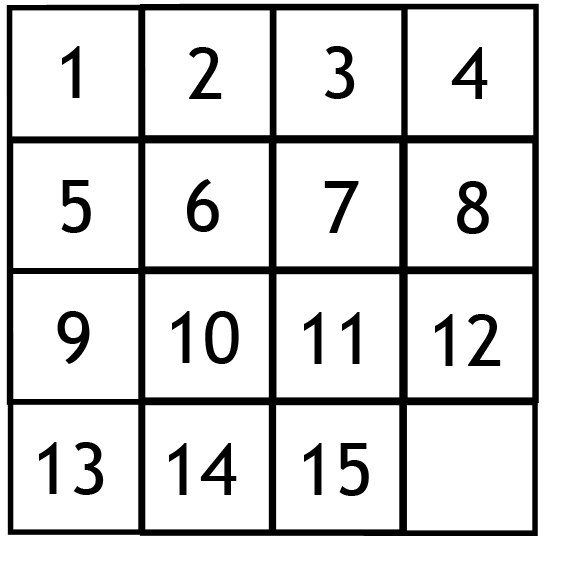
\includegraphics[scale=0.2]{input/pics/MagicPuzzle.png}}
	\hspace{0.02\textwidth}
	\subfloat[\myCaption{Figure of Magic Puzzle with inverse numbers.}]{\label{fig:MagicPuzzleInverse}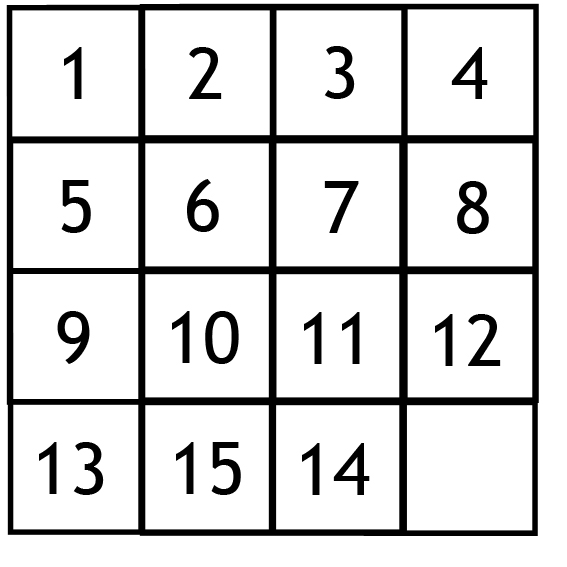
\includegraphics[scale=0.2]{input/pics/MagicPuzzle15-14.jpg}}
	\caption{\myCaption{Illustrations of how the legal and illegal permutations of the Magic Puzzle.}}
	\label{fig:mpuzzles}
\end{figure}

\begin{comment}
	\begin{figure}[!h]
	\begin{center}
	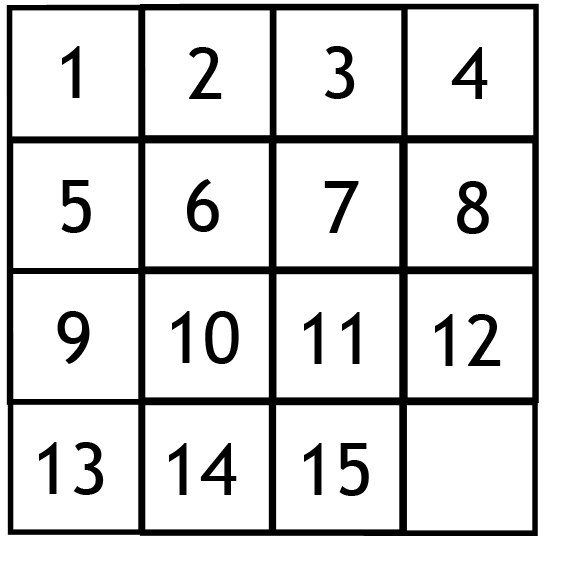
\includegraphics[scale=0.2]{input/pics/MagicPuzzle.png}
	\caption{\myCaption{Figure of Magic Puzzle.}}
	\label{fig:MagicPuzzle}
	\end{center}
	\end{figure}
	
	\begin{figure}[!h]
	\begin{center}
	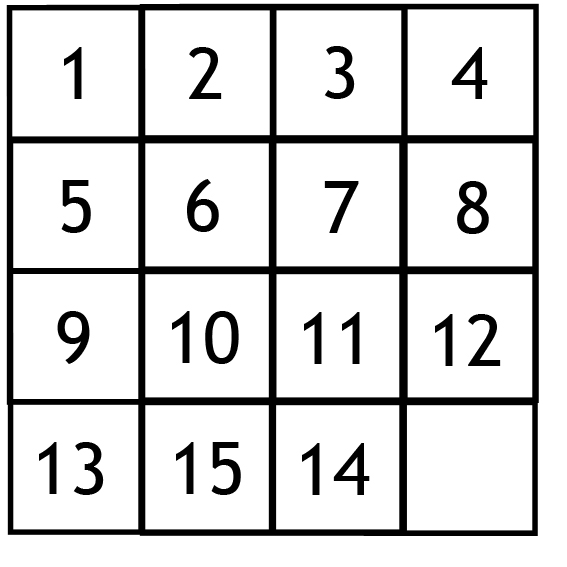
\includegraphics[scale=0.2]{input/pics/MagicPuzzle15-14.jpg}
	\caption{\myCaption{Figure of Magic Puzzle with inverse numbers.}}
	\label{fig:MagicPuzzleInverse}
	\end{center}
	\end{figure}
\end{comment}

For instance we got the figure \ref{fig:MagicPuzzle} and want to switch the tiles to be positioned like on figuare \ref{fig:MagicPuzzleInverse}. This permutation requires an odd transposition of the seven pairs (1,15), (2,14), (3,13), (4,12), (5,11), (6,10) and (7,9). This permutation is not possible because it requires an even number of transpositions to get the empty square at the same position. If we color the contraption like a chess board \ref{fig:Chess} we can see that every odd transposition makes the empty square change color and with every even transposition the empty square lands on a square of the same color.

\begin{figure}[!h]
\begin{center}
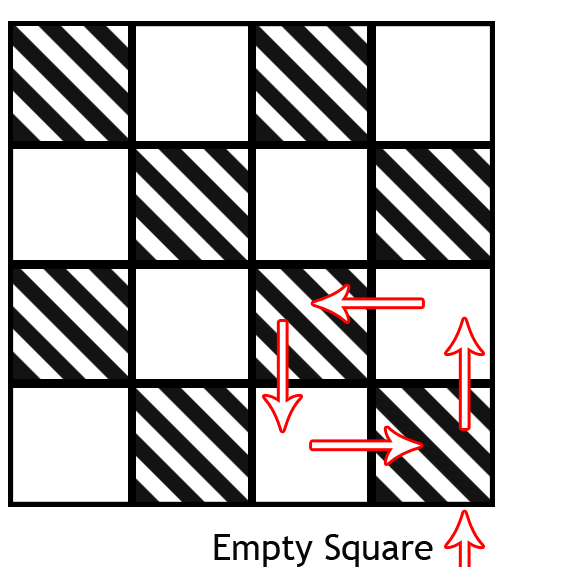
\includegraphics[scale=0.2]{input/pics/MagicPuzzle(EmptySquare).png}
\caption{\myCaption{Figure of Empty Square.}}
\label{fig:Chess}
\end{center}
\end{figure}

Therefore the number of different positions is $\frac{16!}{2}$. But if the empty square has to be in a fixed position then the possible permutations is $\frac{15!}{2}$. These permutations are almost alike the ones the \rubik{} use and they actually inspired \erno{} into his creation of the \rubik{}.